% Created by tikzDevice version 0.12.3.1 on 2021-08-04 23:42:00
% !TEX encoding = UTF-8 Unicode
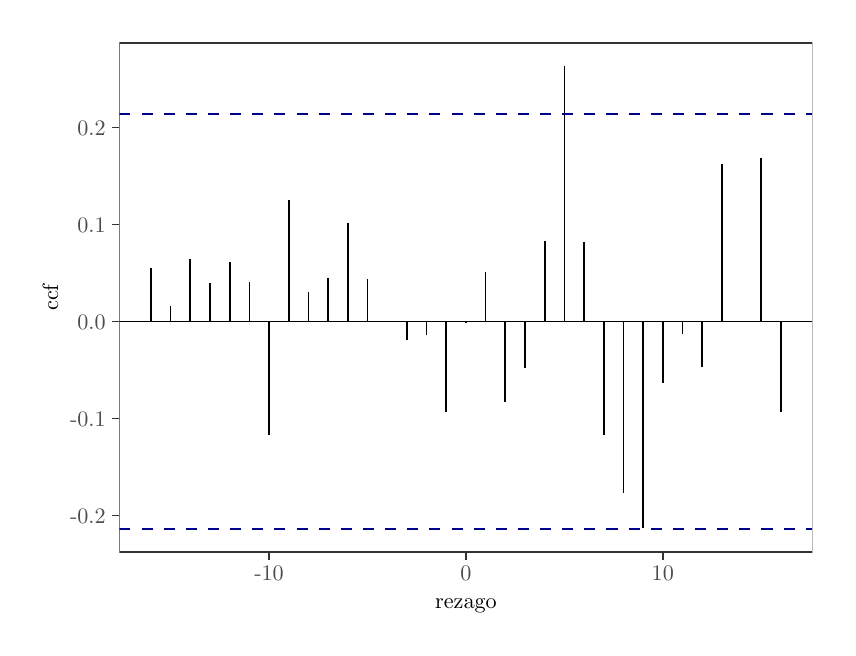
\begin{tikzpicture}[x=1pt,y=1pt]
\definecolor{fillColor}{RGB}{255,255,255}
\path[use as bounding box,fill=fillColor,fill opacity=0.00] (0,0) rectangle (289.08,216.81);
\begin{scope}
\path[clip] (  0.00,  0.00) rectangle (289.08,216.81);
\definecolor{drawColor}{RGB}{255,255,255}
\definecolor{fillColor}{RGB}{255,255,255}

\path[draw=drawColor,line width= 0.6pt,line join=round,line cap=round,fill=fillColor] (  0.00,  0.00) rectangle (289.08,216.81);
\end{scope}
\begin{scope}
\path[clip] ( 33.15, 27.33) rectangle (283.58,211.31);
\definecolor{fillColor}{RGB}{255,255,255}

\path[fill=fillColor] ( 33.15, 27.33) rectangle (283.58,211.31);
\definecolor{drawColor}{RGB}{0,0,0}

\path[draw=drawColor,line width= 0.6pt,line join=round] ( 44.53,129.82) -- ( 44.53,110.65);

\path[draw=drawColor,line width= 0.6pt,line join=round] ( 51.65,116.34) -- ( 51.65,110.65);

\path[draw=drawColor,line width= 0.6pt,line join=round] ( 58.76,133.29) -- ( 58.76,110.65);

\path[draw=drawColor,line width= 0.6pt,line join=round] ( 65.88,124.48) -- ( 65.88,110.65);

\path[draw=drawColor,line width= 0.6pt,line join=round] ( 72.99,132.05) -- ( 72.99,110.65);

\path[draw=drawColor,line width= 0.6pt,line join=round] ( 80.11,124.74) -- ( 80.11,110.65);

\path[draw=drawColor,line width= 0.6pt,line join=round] ( 87.22, 69.56) -- ( 87.22,110.65);

\path[draw=drawColor,line width= 0.6pt,line join=round] ( 94.34,154.71) -- ( 94.34,110.65);

\path[draw=drawColor,line width= 0.6pt,line join=round] (101.45,121.19) -- (101.45,110.65);

\path[draw=drawColor,line width= 0.6pt,line join=round] (108.56,126.53) -- (108.56,110.65);

\path[draw=drawColor,line width= 0.6pt,line join=round] (115.68,146.28) -- (115.68,110.65);

\path[draw=drawColor,line width= 0.6pt,line join=round] (122.79,125.88) -- (122.79,110.65);

\path[draw=drawColor,line width= 0.6pt,line join=round] (129.91,110.34) -- (129.91,110.65);

\path[draw=drawColor,line width= 0.6pt,line join=round] (137.02,103.88) -- (137.02,110.65);

\path[draw=drawColor,line width= 0.6pt,line join=round] (144.14,105.64) -- (144.14,110.65);

\path[draw=drawColor,line width= 0.6pt,line join=round] (151.25, 77.82) -- (151.25,110.65);

\path[draw=drawColor,line width= 0.6pt,line join=round] (158.37,110.00) -- (158.37,110.65);

\path[draw=drawColor,line width= 0.6pt,line join=round] (165.48,128.49) -- (165.48,110.65);

\path[draw=drawColor,line width= 0.6pt,line join=round] (172.59, 81.63) -- (172.59,110.65);

\path[draw=drawColor,line width= 0.6pt,line join=round] (179.71, 93.82) -- (179.71,110.65);

\path[draw=drawColor,line width= 0.6pt,line join=round] (186.82,139.75) -- (186.82,110.65);

\path[draw=drawColor,line width= 0.6pt,line join=round] (193.94,202.95) -- (193.94,110.65);

\path[draw=drawColor,line width= 0.6pt,line join=round] (201.05,139.42) -- (201.05,110.65);

\path[draw=drawColor,line width= 0.6pt,line join=round] (208.17, 69.70) -- (208.17,110.65);

\path[draw=drawColor,line width= 0.6pt,line join=round] (215.28, 48.82) -- (215.28,110.65);

\path[draw=drawColor,line width= 0.6pt,line join=round] (222.40, 35.84) -- (222.40,110.65);

\path[draw=drawColor,line width= 0.6pt,line join=round] (229.51, 88.59) -- (229.51,110.65);

\path[draw=drawColor,line width= 0.6pt,line join=round] (236.62,106.04) -- (236.62,110.65);

\path[draw=drawColor,line width= 0.6pt,line join=round] (243.74, 94.34) -- (243.74,110.65);

\path[draw=drawColor,line width= 0.6pt,line join=round] (250.85,167.37) -- (250.85,110.65);

\path[draw=drawColor,line width= 0.6pt,line join=round] (257.97,110.57) -- (257.97,110.65);

\path[draw=drawColor,line width= 0.6pt,line join=round] (265.08,169.89) -- (265.08,110.65);

\path[draw=drawColor,line width= 0.6pt,line join=round] (272.20, 78.08) -- (272.20,110.65);

\path[draw=drawColor,line width= 0.6pt,line join=round] ( 33.15,110.65) -- (283.58,110.65);
\definecolor{drawColor}{RGB}{0,0,139}

\path[draw=drawColor,line width= 0.6pt,dash pattern=on 4pt off 4pt ,line join=round] ( 33.15,185.61) -- (283.58,185.61);

\path[draw=drawColor,line width= 0.6pt,dash pattern=on 4pt off 4pt ,line join=round] ( 33.15, 35.69) -- (283.58, 35.69);
\definecolor{drawColor}{gray}{0.20}

\path[draw=drawColor,line width= 0.6pt,line join=round,line cap=round] ( 33.15, 27.33) rectangle (283.58,211.31);
\end{scope}
\begin{scope}
\path[clip] (  0.00,  0.00) rectangle (289.08,216.81);
\definecolor{drawColor}{gray}{0.30}

\node[text=drawColor,anchor=base east,inner sep=0pt, outer sep=0pt, scale=  0.80] at ( 28.20, 37.79) {-0.2};

\node[text=drawColor,anchor=base east,inner sep=0pt, outer sep=0pt, scale=  0.80] at ( 28.20, 72.84) {-0.1};

\node[text=drawColor,anchor=base east,inner sep=0pt, outer sep=0pt, scale=  0.80] at ( 28.20,107.90) {0.0};

\node[text=drawColor,anchor=base east,inner sep=0pt, outer sep=0pt, scale=  0.80] at ( 28.20,142.95) {0.1};

\node[text=drawColor,anchor=base east,inner sep=0pt, outer sep=0pt, scale=  0.80] at ( 28.20,178.00) {0.2};
\end{scope}
\begin{scope}
\path[clip] (  0.00,  0.00) rectangle (289.08,216.81);
\definecolor{drawColor}{gray}{0.20}

\path[draw=drawColor,line width= 0.6pt,line join=round] ( 30.40, 40.55) --
	( 33.15, 40.55);

\path[draw=drawColor,line width= 0.6pt,line join=round] ( 30.40, 75.60) --
	( 33.15, 75.60);

\path[draw=drawColor,line width= 0.6pt,line join=round] ( 30.40,110.65) --
	( 33.15,110.65);

\path[draw=drawColor,line width= 0.6pt,line join=round] ( 30.40,145.70) --
	( 33.15,145.70);

\path[draw=drawColor,line width= 0.6pt,line join=round] ( 30.40,180.76) --
	( 33.15,180.76);
\end{scope}
\begin{scope}
\path[clip] (  0.00,  0.00) rectangle (289.08,216.81);
\definecolor{drawColor}{gray}{0.20}

\path[draw=drawColor,line width= 0.6pt,line join=round] ( 87.22, 24.58) --
	( 87.22, 27.33);

\path[draw=drawColor,line width= 0.6pt,line join=round] (158.37, 24.58) --
	(158.37, 27.33);

\path[draw=drawColor,line width= 0.6pt,line join=round] (229.51, 24.58) --
	(229.51, 27.33);
\end{scope}
\begin{scope}
\path[clip] (  0.00,  0.00) rectangle (289.08,216.81);
\definecolor{drawColor}{gray}{0.30}

\node[text=drawColor,anchor=base,inner sep=0pt, outer sep=0pt, scale=  0.80] at ( 87.22, 16.87) {-10};

\node[text=drawColor,anchor=base,inner sep=0pt, outer sep=0pt, scale=  0.80] at (158.37, 16.87) {0};

\node[text=drawColor,anchor=base,inner sep=0pt, outer sep=0pt, scale=  0.80] at (229.51, 16.87) {10};
\end{scope}
\begin{scope}
\path[clip] (  0.00,  0.00) rectangle (289.08,216.81);
\definecolor{drawColor}{RGB}{0,0,0}

\node[text=drawColor,anchor=base,inner sep=0pt, outer sep=0pt, scale=  0.80] at (158.37,  7.06) {rezago};
\end{scope}
\begin{scope}
\path[clip] (  0.00,  0.00) rectangle (289.08,216.81);
\definecolor{drawColor}{RGB}{0,0,0}

\node[text=drawColor,rotate= 90.00,anchor=base,inner sep=0pt, outer sep=0pt, scale=  0.80] at ( 11.01,119.32) {ccf};
\end{scope}
\end{tikzpicture}
